\documentclass{acm_proc_article-sp}
\bibliographystyle{unsrt}

\begin{document}

\title{Cellular Automata for Artificial Life Games}
\numberofauthors{1}
\author{
% 1st. author
%\alignauthor
%Alan S. Wang\\
%       \affaddr{Department of Bioengineering}\\
%       \affaddr{University of California}\\
%       \affaddr{California, Berkeley}\\
% 2nd. author
\alignauthor
Ian Holmes\\
       \affaddr{Department of Bioengineering}\\
       \affaddr{University of California}\\
       \affaddr{California, Berkeley}\\
       \email{ihh@berkeley.edu}
}
\date{30 November, 2013}

\maketitle
\begin{abstract}
An experimental turn-based multiplayer game framework for mobile devices is described.
Using cellular automata, the framework implements models
of condensed-matter physics, mathematical biology,
and the computational study of artificial life.
\end{abstract}

% A category with the (minimum) three required fields
%\category{H.4}{Information Systems Applications}{Miscellaneous}
%A category including the fourth, optional field follows...
%\category{D.2.8}{Software Engineering}{Metrics}[complexity measures, performance measures]


\section{Introduction}

Goal: 
build simulation game for mobile devices,
set in a persistent, multiplayer, computationally-dense world
using cellular automata ({\em CA}),
featuring models from
stochastic physics,
mathematical biology,
 and
artificial computational life ({\em A-Life})

Progress report, describing general structure of platform,
and several models from stochastic biophysics
including simulations of polymer and RNA folding kinetics.

\subsection{Cellular Automata}

CA as a platform for stochastic condensed-matter physics and biophysics
\cite{Schiff2007}

CA as a general platform for games
\cite{SimCity,DwarfFortress,Minecraft}
and electronic toys or art \cite{RuckerCAPOW,PowderToy}

\subsection{Artificial Life Models}

Electronic
\cite{VonNeumannBook,Wireworld}

Macro-biological
\cite{ConwaysLife,Langton1986}

Kinematic
\cite{Stevens2011}

Genetic algorithms
\cite{Tierra,Avida}

Core War
\cite{CoreWarGuidelines84,CoreWarDewdney85,BarkleyWaitSchmidtCoreWar2004}

\subsection{Molecular Evolution Models}

One of the best-studied models of the origin of life is the ``RNA World''
\cite{Woese1967}.
Life within vesicles, or concentrated in favorable environments such as hydrothermal vents.  % define 'vesicle', 'micelle'
Spatial concentration of polymer information tapes whose chemistry naturally favors self-replication.
Micelles.

Synthetic RNA World systems
\cite{PaulJoyce2002}

RNA A-Life
\cite{journals/alife/Schuster94}

RNA Folding on Lattice
\cite{LeoniVanderzande2003,JostEveraers2010,ZaraPretti2007,GillespieMayneJiang2009}

Protein folding on the lattice. HP model \cite{Dill1985,PandeRokhsar1999}

\section{Simulation}

Pixel Zoo.
Architecture of underlying Cellular Automata platform, called ``Zoo Gas''.

Board:
Square slab of cubic lattice, dimensions $S \times S \times D$.
Assuming 64-bit architecture (upper limit of 128 bits/cell, ignoring rare scripted agent cells), requires $16S^2 D$ bytes.

General idea is to expose a low-level fast machine for majority usage during play,
with high-level functional language (Scheme) available for occasional in-game scripting usage.

\subsection{Low-Level Virtual State Machine}

Low-level (machine code):
state machines.

Synchronized and asynchronous callback.
Asynchronous guarantees callback with an exponentially-distributed wait time, scaled by particle's update rate.
Random number generator is Mersenne twister, built into board, and is replayable.

Addressing: local neighborhood.
Memory structure: 64 bits of state per cell, plus a pointer to opaque storage (can only be accessed via the supervisor scripting language).

Main 64-bit state divided into bitfields. 16 bits given over to a type field, determining how cell will be updated.
Remaining 48 bits used as dynamic storage; division into bitfields depends on the type, with some universal restrictions (e.g. bitfields cannot straddle a 32-bit boundary).
Supplemented by larger amount of read-only global storage (including global program).

The 16-bit type field selects the global program to update the cell and its neighborhood,
and also specifies a naming and sizing scheme for bitfields associated with that type's use of the dynamic storage in that cell.

The global program for a state machine generalizes the concept of the state lookup table to facilitate partial matching and rewriting of bitfields in the local lattice neighborhood.
The virtual machine resembles an ultra-minimal subset of a typical CISC register-machine architecture.
The instruction set is low-level, recognizably close to ARM\cite{seal00} and not too far from Core War's RedCode\cite{CoreWarGuidelines84}.
The instructions can be quickly interpreted from or implemented in C, and will be optimized reasonably well by C compilers.
Such details of the implementation are left opaque by design.
Code written for the low-level state machine cannot reflect on or modify its own global program.

{\bf INSTRUCTION SET} The following minimalistic operations may be easily interpreted
or compiled to C (using {\tt switch}, {\tt if}, {\tt goto})
or directly to a RISC instruction set like ARM\cite{seal00}
(using {\bf LDR}, {\bf STR}, {\bf ADD}, {\bf SUB}, {\bf B}).
Operands and bitfield addresses may be specified as literal constants (immediate addressing mode), or by registers (indirect addressing mode).
The available instructions are
\\
{\bf Load-Add-Store} This operation encapsulates writes: loads a value from a source bitfield address, adds an operand to it, stores result in a destination bitfield address. Can optionally move or destroy the opaque storage.
\\
{\bf Load-Compare-Branch} This op encapsulates memory reads. Reads from a local bitfield address, compares value to an operand, branches conditionally based on comparison.
\\
{\bf Load-Switch} Analogous to C's {\tt switch}: loads a bitfield from memory, dispatches based on value. Can be implemented using {\bf Load-Compare-Branch}, or a jump table.
\\
{\bf Load-Register} Places a numeric constant into a temporary register. Used in combination with indirect addressing modes of other instructions.
\\
{\bf Branch-Goto} Forward-branch to labeled routine.
\\
{\bf Branch-Random} Forward-branch conditional on a bit from the random number generator.
\\
{\bf Branch-Neighbor} Branch to labeled entry point in neighbor's program (restricted to supervisor).
\\
{\bf Call-Script} calls a Scheme function (restricted to supervisor).

Control flow is monotonic: goto is one-way, there is no stack, no gosub or return keywords.
Branches always go forward, so loops are explicitly prohibited.
Any program is a Directed Acyclic Graph (DAG) of finite determinable length.
It is easy for a server to analyze player-designed programs and maintain strong performance guarantees.
There is enough flexibility for players to implement novel material properties in the CA,
as well as more sophisticated computational behaviors (e.g. Turing machines, Langton ants, Wireworld-type circuits).

\subsubsection{Addressing Modes}

Several addressing modes for memory locations and operands.

Immediate vs register addressing (operands).

Indirect addressing (memory access). Registers specify cell offset, bitfield sub-address.

In principle do not need indirect or register addressing: can explicitly enumerate all cases via immediate addressing.
In practice, useful to allow some indirect and register addressing, to reduce program sizes via re-use of subroutine code.

Indirect addressing (code execution).
{\bf Branch-neighbor}: effectively a primitive message delivery mechanism.
Must be restricted as it can create loops.

\subsubsection{Assembly Language}

Low-level (assembly language):
Scheme. Generates (assembles) instructions for state machine.

Large built-in library for replicating patterns over Moore or von Neumann neighborhoods,
implementing reaction-diffusion models, implementing turtle-type agents, etc.

Selected functions from this library are exposed to the player,
to facilitate game design (e.g. diffusions, turtles) and reduce program sizes.

\subsection{Higher-Level Functions}

As well as being used at assembly time to specify macros,
Scheme functions can be invoked dynamically by the virtual state machine for higher (supervisory-level) functions involving path-finding, goal-satisfaction, and other agent- and game-level scripting.
These features are restricted to game designers.

An optional S-expression can be associated with any cell for dynamic storage associated with the agent scripts.
This storage is opaque to state machine: there is one instruction ({\bf Load-Add-Store}) that, when rewriting the type field, is allowed to destroy the S-expression associated with a cell, or it can move it to a neighboring cell.
Other than this, the low-level machine may not copy, create, read or modify cell S-expressions.
In contrast, the Scheme supervisor has access to the state machine environment, board API, and multiplayer client API.

The polymers, RNA molecules, and other models described here (including ``Agent State Machines'') do not require Scheme scripting, only Scheme assembly language generation (which is a one-time cost).

\subsection{Polymer State Machines}

Polymers fundamental to modeling thermodynamically fluctuating enclosures like micelles.
Also to modeling biological polymers: RNA and proteins.

Theoretical physics \cite{DoiEdwards1988} and CA simulation of polymers \cite{PhysRevLett.64.1915,journals/pc/OstrovskyCSB01}

As shown in Figure~\ref{fig:polymer}.

\begin{figure}
\fbox{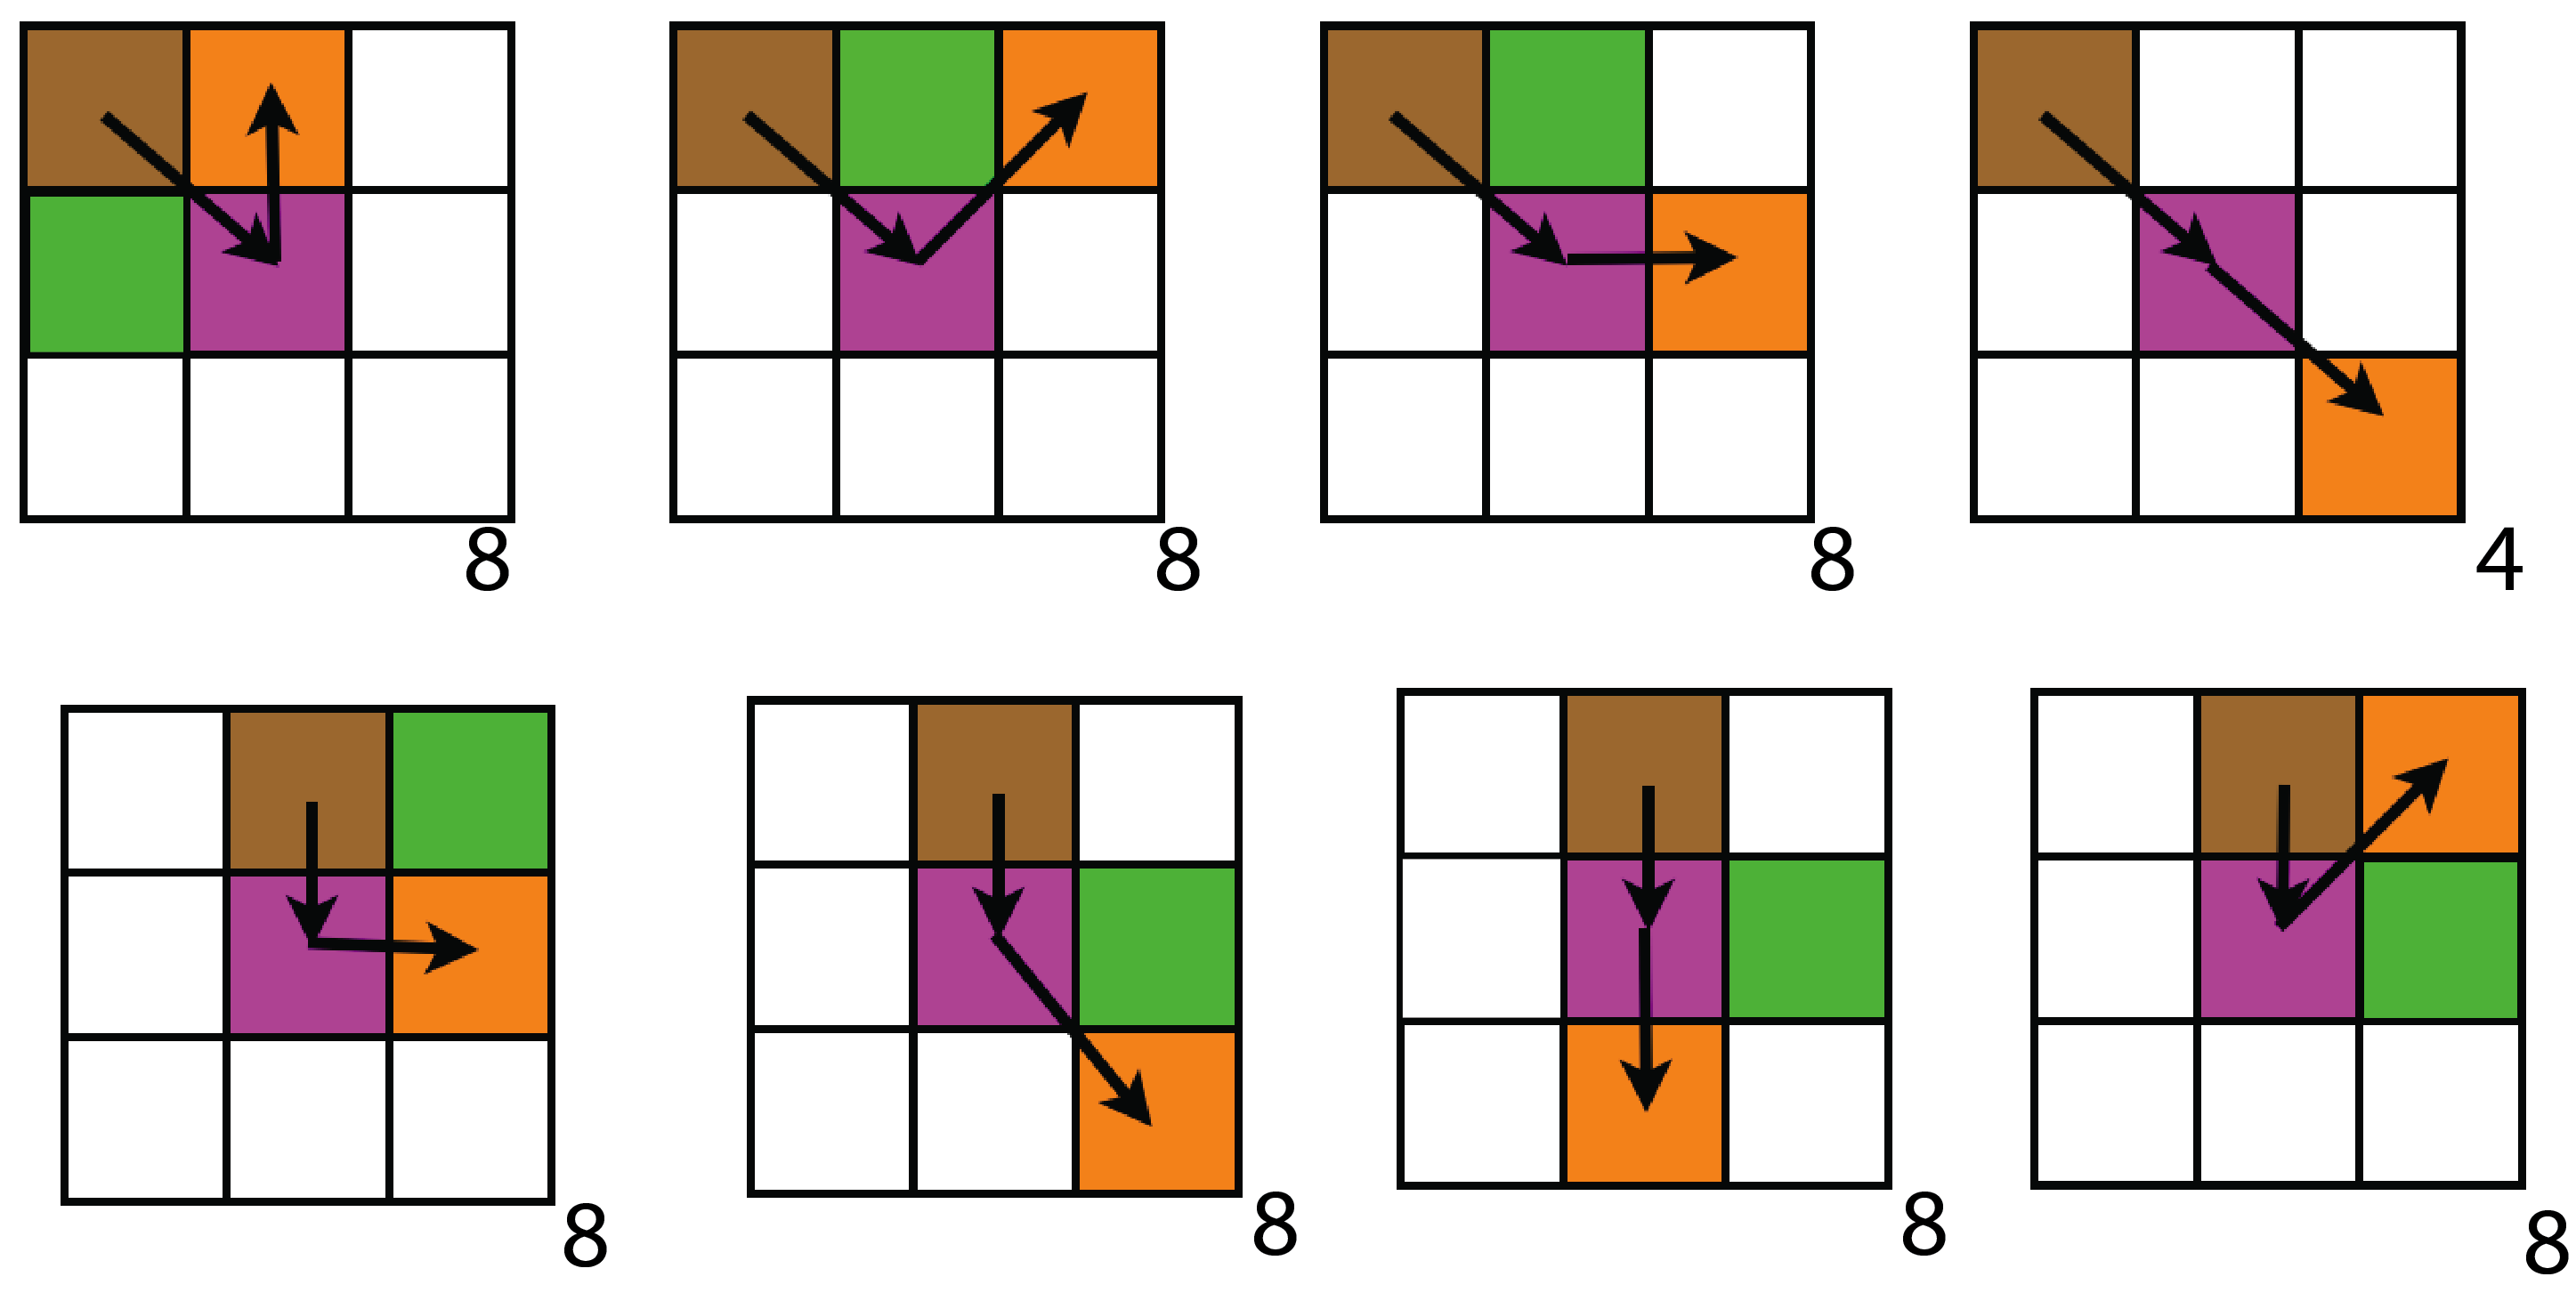
\includegraphics[width=\columnwidth]{Polymer.png}}
\caption{
\label{fig:polymer}
A few cases in the explicit automata-theoretic enumeration of polymer diffusion on the square lattice.
}
\end{figure}

Number of states, theoretical.

Real-world implementation.
Lookup/modify, no indirect addressing (closest thing to state tables): 2.3Mb.
Only 52k gzipped (still vicious to expand).
With indirect addressing: down to 127k (gzipped: 3k).
Scheme generator is 5k (gzipped: 1k).


\subsection{RNA State Machines}

RNA on a lattice \cite{LeoniVanderzande2003,JostEveraers2010,ZaraPretti2007,GillespieMayneJiang2009}


As shown in Figure~\ref{fig:rna}.

\begin{figure}
\fbox{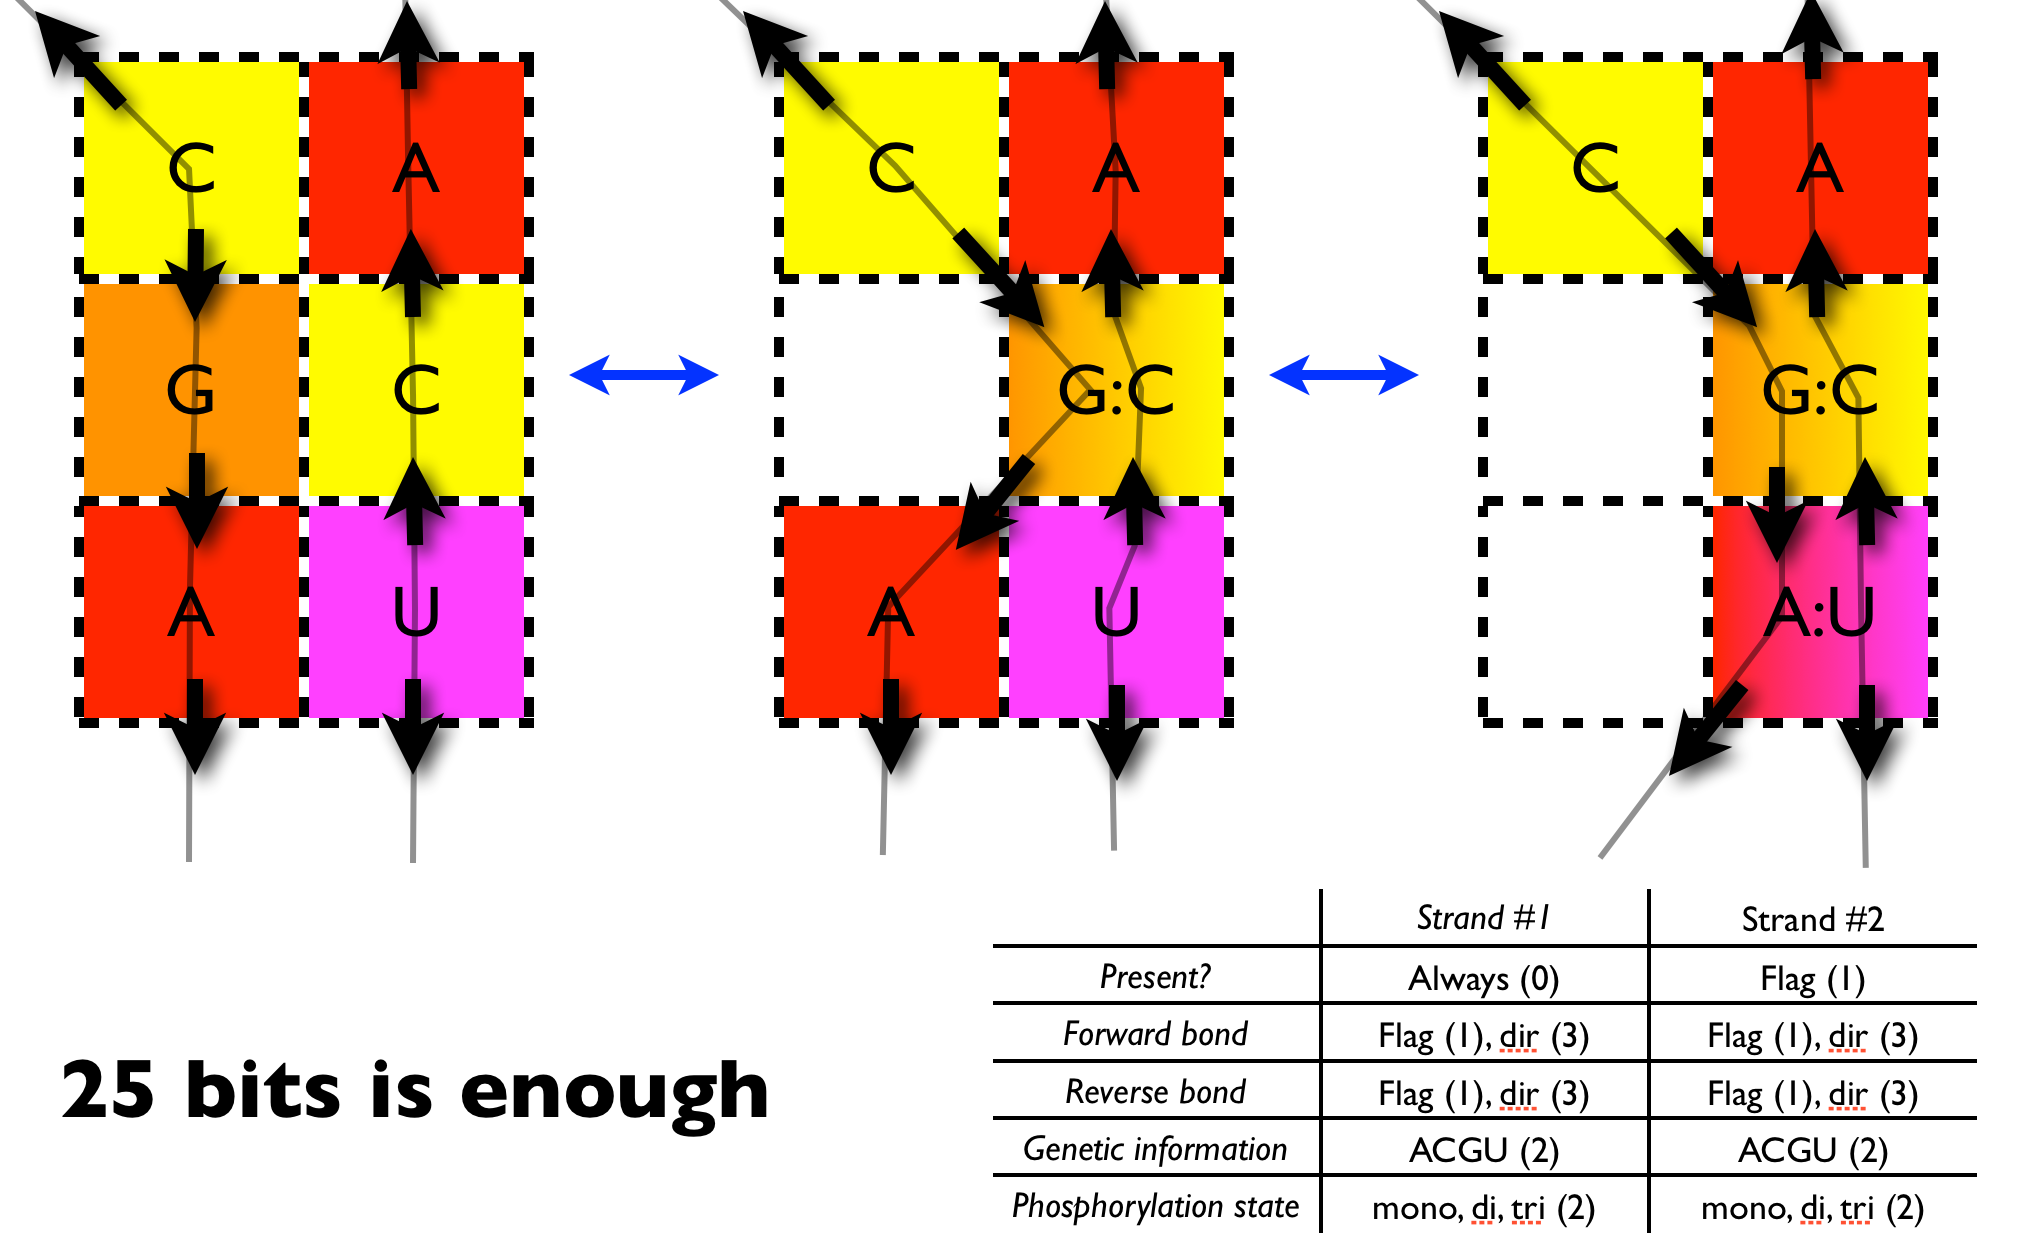
\includegraphics[width=\columnwidth]{RNA.png}}
\caption{
\label{fig:rna}
A sample case in the explicit automata-theoretic enumeration of RNA folding on the square lattice.
}
\end{figure}

Number of states, theoretical.


\subsection{Agent State Machines}

Pixel Zoo also implements various agent models from above molecular length scale, used in game design.

Tumble-run: {\em E.coli}.
\cite{RosserEtAl2013}

%Sudoku ant: push obstacle a random number of blocks before changing direction.
%\cite{AntBehaviorNature}

Reaction-diffusion.
Directed diffusion.
Diffusion-limited aggregation.
\cite{DLA}

Two-dimensional square-lattice Ising model \cite{Onsager1944}.

Lotka-Volterra (predator-prey) \cite{Lotka1910,Hirota199739}.
Rock-paper-scissors games in ecology \cite{Tainaka2000}.

Ecosystem balancing and stability of food webs \cite{quince2005topological}.

Forest fires \cite{Karafyllidis1997}.

Population dynamics and spatial versions of the Wright-Fisher model \cite{MathiesonMcVean2013}.

\subsection{Rendering}

Isometric view.
Sprites, tiles.

\section{Game Design}

\subsection{Basic Play}

Terraforming simulation.
Isometric PAINT with live pixels.

Game goal: maintain dynamic equilibrium between three RPS species within a vesicle.

\subsection{Network Play}

Multiplayer implementation: RESTful server \cite{rest}.
Post lock, check board out/in.

Time-limited turns, minimum time between turns, max tool recharge per day.

Multiplayer goal: keep your population alive under attack.

Earn game-money from your population.

Client: log in/out, browse worlds, pick a world, select terraforming tools...

\subsection{Creating New Tools}

Player can POST XML to server describing new particles and tools
(with restrictions, e.g. no Scheme code at present, due partly to prohibitions on Turing-complete code transfer by App Store owners).

Spend game-money creating and using new reaction-diffusion particles and spray-tools.

Earn game-money when others buy your tools.

\subsection{Implementation}

Gnu C, libXML, GDataXML, ChibiScheme, XCode, Catalyst (Perl).

RNA state machines implemented in Java prototype.

\section{Discussion}

Work in progress.

\subsection{Acknowledgements}

Many thanks are due Alex Shinn, Richard Evans, Michael Mateas, Sean Eddy, Gerald Joyce, Chris Quince,
and Rudy Rucker for help and inspiration.


\bibliography{pzpaper}

\balancecolumns
% That's all folks!
\end{document}
